\clearpage
\section{Systeme}
\subsection{Eigenschaften}
\begin{enumerate}
\small
  \item{\textbf{Speicher}}\\
      % \begin{mdframed}[style=exercise]
          \textbf{-frei}: Vollständige Beschreibung durch xy-Kennlinie, Ausgang $y(t=t_0)$ nur von aktuellen Eingangswerten $x(t=t_0)$ abhängig $\rightarrow$ gedächtnislos.\\
          \[
              \text{z.B. \ }y(t)=\frac{R_1}{R_1+R_2}\cdot x(t)
          \]
          \textbf{-behaftet}: Ausgang inkl. vergangene Werte, keine vollständige Beschreibung durch xy-Kennlinie.\\
          \[
              \text{z.B. \ }y(t) = x(t)\cdot 2x(t-1)
          \]
      % \end{mdframed}
  \item{\textbf{Kausalit\"at}}\\
      % \begin{mdframed}[style=exercise]
           Ausgang $y(t=t_0)$ hängt nur von aktuellen + vorherigen
           Eingangswerten $x(t\le t_0)$ ab. Keine Zukunftswerte! \\
           Impulsantwort $h(t)$ beginnt ab $t=0: t<0 \rightarrow h(t)=0$.
          \[
              \text{z.B.\ }y(t) =
              \int\displaylimits_{t-5}^{t}x(\tau)d\tau
          \]
      % \end{mdframed}
 Aus Speicherfreiheit folgt Kausalität, \underline{nicht} umgekehrt.
 \textbf{Kausale} gebr. rationale Fkt.: Nennergrad $\ge$ Zählergrad.
 
  \item {\textbf{(BIBO-)Stabilit\"at}}\\
  \small BIBO: beschr\"ankter Eingang $\rightarrow$ beschr\"ankter Ausgang.\\
  %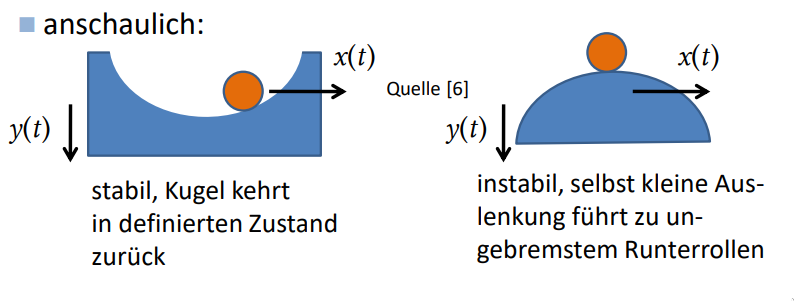
\includegraphics[width=.9\columnwidth]{Systeme/BIBO_anschaulich}\\
\begin{mdframed}[style=exercise]
   System ist \textbf{stabil}, wenn
   \begin{itemize}
   	   \item $h(t)$ absolut integrierbar ist: $\int_{-\infty}^{\infty} |h(t)| dt <\infty$
   	   \item P/N-Diagramm: \textbf{alle} Pole links der $\omega$-Achse
   	   \item gebr. rationale Fkt.: Nennergrad $\ge$ Zählergrad
   	   \item \textit{zeitdiskret (ZD)}: EK $\in$ Kb
   	   \item \textit{ZD}: alle Pole innerhalb
   	   des EK
   	    \item \textit{ZD}: absolut summierbar: $\sum_{n=-\infty}^{\infty} |h(n)|<\infty$
   \end{itemize}
   z.B.: $y(t) = 50\cdot x^3(t)$, instabil: $y(t) = e^{t}\cdot x(t)$
  \end{mdframed}
  \normalsize
  \item{\textbf{Zeitinvarianz}}\\
		{\small
		  	Eingang zeitverschoben $\rightarrow$ Ausgang zeitverschoben.
		}
		\[ 
		x(t-t_0) = y(t-t_0)
		 \]
		 
		 {\small z.B. $y(t)=t\cdot \sin(t)$}
  \item{\textbf{Linearit\"at}}\\
		  {\small
		      Lineares System: Superpositionsprinzip gilt $\rightarrow$ siehe Ausblendeeigenschaft, Zerlegung in gerades/ungerades Signal.
		  }
\end{enumerate}
\normalsize
\subsection{LTI-Systeme}
\subsubsection{Beschreibung}
LTI-Systeme: Linear, Zeitinvariant (time-invariant).\\
Operatoren: $+, -, \frac{d}{dt}, \int, t-t_0$ (Verz\"ogerung)\\

Beschreibung des Ein- und Ausgangsverhalten im
\begin{itemize}
	\item Zeitbereich $x(t)$: DGL, Signalflussplan, Impulsantwort
	\item Frequenz- $\underline{X}(\omega)$ bzw. Bildbereich $\underline{X}(s)$: Übertragungs-Fkt., Frequenzgang, Bode- und P/N-Diagramm.
\end{itemize}
\subsubsection{Differenzialgleichung (DGL)}
\begin{itemize}
	\small
	\item Bestimmung Eingangs-/Ausgangsgr\"o\ss en der Schaltung.
	\item Gleichgewicht: Maschengleichung für $u$,\par Knotengleichungen f\"ur $i$ aufstellen.
	\item DGL enth\"alt nur Konstanten ($C,L$), $u$ bzw. $i$ in der Grundform und beliebiger Ableitung (bzw. deren Integrale). Integrale durch Ableiten eliminieren.
	\item $u,i$ durch Systemgr\"o\ss en mithilfe von Bauteilgleichungen ausdr\"ucken, Schaltung beachten!
	\normalsize
	\item Bauteil-/Zweipolgleichungen:
	\begin{gather*}
		u_R = R \cdot i \quad \boxed{i_c = C \cdot \frac{du_C}{dt}} \quad \boxed{u_L = L \cdot \frac{di_L}{dt}}
	\end{gather*}
	\item DGL 2.Ordnung allgemein:
\begin{gather*}
		\underbrace{a_2 \ddot{x}_a + a_1 \dot{x}_a + a_0 x_a}_{\texttt{Ausgangsgr\"o\ss en}} = \underbrace{b_2 \ddot{x}_e + b_1 \dot{x}_e + b_0 x_e}_{\texttt{Eingangsgr\"o\ss en}}
\end{gather*}
\end{itemize}

\subsubsection{Impuls \& Sprungantwort}
\small
\begin{centering}
	\setlength{\abovedisplayskip}{-10pt}
	\setlength{\belowdisplayskip}{-5pt}
	\begin{tabularx}{\columnwidth}{|X|X|}
		\hline
		Impulsanregung & Impulsantwort\\
		\hline
		$x(t)=\delta(t)$ & $y(t)= h(t) = S\{ \delta(t) \}$ \\
		\hline
		{
			\begin{align*}
				x(t) &= \int_{-\infty}^{\infty}x(\tau) \cdot \delta(t-\tau) \, d\tau\\
				\delta(t) &= \frac{d}{dt} \, \varepsilon(t)
			\end{align*}
		}	 &
		{
			\begin{align*}	
				y(t) &= \int_{-\infty}^{\infty}x(\tau) \cdot h(t-\tau) \, d\tau\\
				&= x(t) * h(t)\\
				h(t) &= \frac{d}{dt} \, g(t)
			\end{align*}
		}	\\
		\hline\hline
		Sprunganregung & Sprungantwort \\
		\hline
		$x(t)=\varepsilon(t)$ & $y(t)= g(t) = S\{ \varepsilon(t) \}$ \\
		\hline
		{
			\begin{align*}	
				\varepsilon(n) &= \int_{-\infty}^{\infty} \delta(t) \, dt
			\end{align*}
		} &
		{
			\begin{align*}	
			g(t) &= \int_{-\infty}^{\infty} h(t) \, dt
			\end{align*}
		}\\
		\hline
	\end{tabularx}
\end{centering}
\normalsize
\subsubsection{Faltung}
\small
Aus $h(t)$ eines LTI-Systems und Eingang $x(t)$ lässt sich
Ausgang $y(t)$ durch Faltung bestimmen:
\normalsize
  \[
      y(t) = \int_{-\infty}^{+\infty} x(\tau)\cdot h(t-\tau)d\tau = \boxed{x(t)*h(t)}
  \]
  \begin{itemize}
  	  \item $\delta(t)$: \underline{neutrales} Element der Faltung
  	  \[
  	  x(t)* \delta(t) = x(t)
  	  \]
  	\item Faltung mit verschobenen Dirac-Impuls \\$\rightarrow$ Verschiebung des Signals:
  	\[
  	x(t)* \delta(t - t_0) = x(t - t_0)
  	\]
  \end{itemize}

\begin{mdframed}[style=exercise,frametitle=Rechenregeln]
  \begin{itemize}
	\item {$a*b=b*a$} {\small \qquad kommutativ}
	\item $a*[b*c]=[a*b]*c$
	\item $a\cdot(f*g)=(a\cdot f) * g = f * (a\cdot g)$
	\item $a*[b+c]=a*b+a*c$
  \end{itemize}
\end{mdframed}
\clearpage
\subsection{Frequenzgang}
  \begin{itemize}
      \item{\textbf{Frequenzgang}}\\
          \[
              \underline{H}(\omega) = \frac{1}{\underline{A}_{11}} =
              \frac{\underline{Y}(\omega)}{\underline{X}(\omega)} =
              \frac{\underline{U_2}(\omega)}{\underline{U_1}(\omega)} = |\underline{H}(\omega)|\cdot e^{j\varphi_H(\omega)}
          \]
      \item{\textbf{Amplitudengang}}, Betragsfrequenzgang
      
      {\small LTI-System ändert Eingangssignal um Faktor $A(\omega)$}.
          \[
              A(\omega) = |\underline{H}(\omega)| =
              \frac{|\underline{Y}(\omega)|}{|\underline{X}(\omega)|}
              \begin{cases}
                  > 1 & \text{Verst\"arkung}\\
                  < 1 & \text{D\"ampfung}
              \end{cases}
          \]
      \item{\textbf{Phasengang}}, Phasenfrequenzgang\\
          \[
              \varphi_H(\omega) = \text{arg}\{\underline{H}(\omega)\} =
              \varphi_Y(\omega) - \varphi_X(\omega)
          \]
          \[
              \varphi_H = \text{arctan}\left(\frac{\mathfrak{Im}}{\mathfrak{Re}}\right)
          \]
  \end{itemize}
  \subsection{Übertragungsfunktion (Ü-Fkt.)}\label{ufkt}
  \begin{itemize}      
      \item{\textbf{Eigenfunktion}}\\
          \[
              y(t) = \lambda\cdot x(t)
              \begin{cases}
                  x(t): & \text{Eigenfunktion}\\
                  \lambda: & \text{Eigenwert}(\lambda\in\mathbb{C})
              \end{cases}
          \]
            Jede komplexe Exponentialfunktion $x(t) = \e^{st}$ ist\\ Eigenfunktion
          jedes beliebigen LTI-Systems $S$:
          \[
          y(t) = S\left\{ \e^{st} \right\} = \lambda\cdot \e^{st}
          \]
          \[
          \lambda = \underline{H}(s) = \int_{-\infty}^{+\infty} h(\tau)\  \e^{-st} d\tau
          \]
  \end{itemize}

  \begin{itemize}\small
      \item{\textbf{Erweiterung der KWR}}
      
      KWR: komplexe Wechselstromrechnung. \\
          Die harmonische Exponentialfunktion $e^{j\omega t}$ ist ein
          \\Sonderfall von $e^{st}$ mit $s=j\omega+\sigma$, wenn $\sigma=0$.
          \[
              \sigma \triangleq \text{Amplitude}
              \begin{cases}
                  \sigma \leq 0 & \text{exponentiell abklingend}\\
                  \sigma = 0 & \text{konstante Amplitude}\\
                  \sigma \geq 0 & \text{exponentiell zunehmend}
              \end{cases}
          \]
          \[
              \omega \triangleq \text{Rotation}
              \begin{cases}
                  \omega \leq 0 & \text{Zeiger rotiert mit UZS}\\
                  \omega = 0 & \text{Zeiger rotiert nicht}\\
                  \omega \geq 0 & \text{Zeiger rotiert gegen UZS}
              \end{cases}
          \]
          \normalsize
  
% \[
%   \boxed{
%   \begin{circuitikz}[scale=1,transform shape]
%       \draw(0,0) to[generic] node[anchor=east,yshift=-20pt]{$\underline{Z}(s)\mathrm{=}R$} (2,0);
%       \draw(3,0) to[L] node[anchor=east,yshift=-20pt, xshift=5pt]{$\underline{Z}(s)\mathrm{=}s\cdot L$} (5,0);
%       \draw(6,0) to[C, l=] node[anchor=east, yshift=-20pt, xshift=6pt]{$\underline{Z}(s)\mathrm{=}\frac{1}{s\cdot C}$} (8,0);
%   \end{circuitikz}
%   }
% \]

\item \textbf{komplexe \"Ubertragungsfunktion}
  \footnotesize
  \[
      \underline{H}(s)=\frac{\underline{Y}(s)}{\underline{X}(s)}=\frac{\underline{U_2}(s)}{\underline{U_1}(s)}=\frac{\text{komplexer
      Zeiger Ausgang}}{\text{komplexer Zeiger
      Eingang}}
  \]
  \normalsize
  Übertragungsfunktion $H(s)$ mit komplexer Frequenz
  $s=\sigma+j\omega$ $\rightarrow$ Ersetze $jw$ durch $s$.
\end{itemize}
  
\subsubsection{Gebrochen-rationale Ü-Fkt.}
{\small Grad \textbf{N} des Nennerpolynoms: Ordnung des LTI-Systems =\\ Anzahl unabhäng. Energiespeicher ($L, C$). \\
\textbf{Kausales} System, wenn Nennergrad $N\ge M$ Z\"ahlergrad}.
\[
H(s)=\frac{\sum_{m=0}^{M} b_{m} \cdot s^{m}}{\sum_{n=0}^{N} a_{n} \cdot s^{n}}
\]
Beispiel: DGL 2.Ordnung im Zeitbereich:
\[
a_2\ddot{y}(t)+a_1\dot{y}(t)+a_0 y(t)=b_2\ddot{x}(t)+b_1\dot{x}(t)+b_0 x(t)
\]
$\rightarrow$ Ü-Funktion im Bildbereich (System 2.Ordnung):
\[
\underline{H}(s)=\frac{\underline{Y}(s)}{\underline{X}(s)}=\frac{b_2 s^2+b_1 s+b_0}{a_2 s^2 +a_1 s +a_0}
=\frac{b_2 s^2+b_1 s+b_0}{a_2 s^2 +a_1 s +a_0}
\]
\subsection{Pol-Nullstellen-Diagramm}\label{pn_diagramm_systeme}
{\small Grafische Darstellung der s-Ebene. (siehe Kap. \ref{pn_diagramm_lpt})\\
$K$: Maßstabs-/Verstärkungsfaktor.}
	\[
	 \underline{H}(s) =\frac{b_M}{a_N} \frac{\prod_{o=1}^{M} (s-z_o)}{\prod_{x=1}^{N} (s-z_x)} \text{ mit } K=\frac{b_M}{a_N}
	\]
\begin{itemize}
\item Achsen: Im\{$s$\} = $\omega$, \quad Re\{$s$\} = $\sigma$
\item Kausalität: Nennergrad $N$ $\ge$ Zählergrad $M$.
\item \textbf{Alle} Pole links der $\omega$-Achse: \textbf{stabiles} + \textbf{kausales} LTI-System.
\item Pole \& Nullstellen sind entweder reell (nur auf Re-Achse) oder \textbf{paarweise} komplex-konjungiert.
\end{itemize}
\subsubsection{Frequenzgang aus dem P/N-Diagramm}\label{fgang_pn}
      \small{$\underline{H}(\omega)$ existiert nur, wenn im PN-Diagramm $\omega$-Achse $\in$ Kb (siehe Kap. \ref{pn_diagramm_lpt}) bzw. alle Pole links der $\omega$-Achse (stabiles System).} \\
      
\textbf{Näherungsweise} Bestimmung:
\begin{itemize}
\item An der $\omega$-Achse von 0 nach oben entlang gehen.
\item Polstelle: \textbf{Maxima}/Erhöhung im Amplitudengang.
\begin{itemize}
	\item PST nah an s-Ebene: hohe Totzeit, dominant.
	\item \textbf{stabiler} Pol: links der $\omega$-Achse.
	\item PST im Ursprung: Verhalten $\rightarrow$ ideales \textbf{I-Glied}:\\ Bode: $-20dB$/Dek., $\varphi=-$ 90\textdegree.
\end{itemize}
\item Nullstelle: \textbf{Minima}/Absenkung im Amplitudengang.
\begin{itemize}
	\item Nullstelle (NST) auf $\omega$-Achse: NST im Amplitudengang.
	\item NST im Ursprung: Verhalten $\rightarrow$ ideales \textbf{D-Glied}:\\ Bode: $+20dB$/Dek, $ \varphi=+$ 90\textdegree.
\end{itemize}

\end{itemize}
\textbf{Genaue} Bestimmung:
\begin{itemize}
	\item An der $\omega$-Achse von 0 nach oben entlang gehen.
	\item Jede Pos. auf $\omega$-Achse: Längen und Winkel der kompl. Zeiger $c_{o,i}$ und $c_{zp,i}$ messen mit Geodreieck.
	\[
	|\underline{H}(\omega)|=\frac{\prod_{o=1}^{M}\text{alle Längen } |c_o,i|}{\prod_{p=1}^{N}\text{alle Längen } |c_p,i|}
	\]
	\[
	\varphi_H(w)=(\text{Summe } \angle \underline{c}_{o,i}{\omega})-(\text{Summe } \angle \underline{c}_{p,i}{\omega})
	\]
\end{itemize}
\textbf{Minimal}phasiges System:
\begin{itemize}
	\item Alle NST links der $\omega$ und $\sigma$-Achse.
	\item Sehr geringe Phasen\"anderung \"uber Frequenz.
	\item Geringe Signalverz\"ogerung.
\end{itemize}

\clearpage
\subsection{Zusammenschaltung LTI-Systeme}
\begin{itemize}
    \item \textbf{Kettenschaltung}\\
        \textit{Produkt} der Ü-Fkt. der Einzelsysteme.
        \[
            \boxed{\underline{H}_{e}(s)=\underline{H}_{B}(s) \cdot \underline{H}_{A}(s)=\underline{H}_{A}(s) \cdot \underline{H}_{B}(s)}
        \]
        \begin{center}
            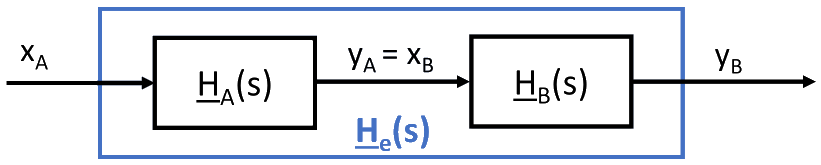
\includegraphics[width=0.7\columnwidth]{Kettenschaltung_Uebertragungsglieder}
            \[
                \underline{Y}_{B}=\underline{H}_{B}(s) \cdot \underline{X}_{B}=\underline{H}_{B}(s) \cdot \underline{Y}_{A}=\underline{H}_{B}(s) \cdot \underline{H}_{A}(s) \cdot \underline{X}_{A}
            \]
        \end{center}
        \begin{itemize}
	        \item Voraussetzung: Rückwirkungsfreiheit (mit Trennverstärker) zwischen $\underline{H}_A(s)$ und $\underline{H}_B(s)$.
        	\item \textbf{Bodediagramm}: \textit{Addition} der einzelnen Glieder beim Amplituden- und Phasengang.
        \end{itemize}      
    \item \textbf{Parallelschaltung}\\
        \textit{Summe} der einzelnen Ü-Glieder.
        \[
            \boxed{\underline{H}_{e}(s)=\underline{H}_{B}(s) + \underline{H}_{A}(s)}
        \]
        \begin{center}
            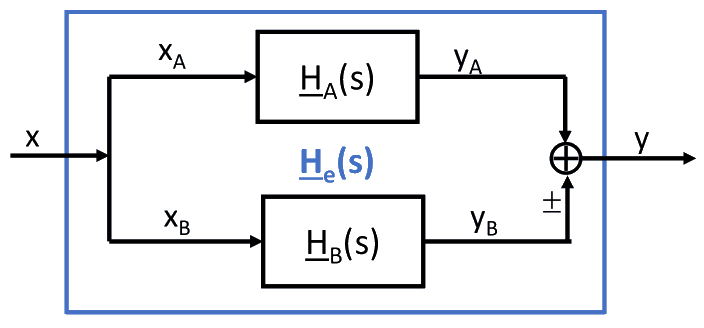
\includegraphics[width=0.6\columnwidth]{Parallel_Uebertragungsglieder}
            \begin{align*}
                \underline{Y}&=\underline{Y}_{A} \pm \underline{Y}_{B}\\
                             &=\underline{H}_{A}(s) \cdot \underline{X}_{A} \pm \underline{H}_{B}(s) \cdot \underline{X}_{B}\\
                             &=\left(\underline{H}_{A}(s)+\underline{H}_{B}(s)\right) \cdot \underline{X}
            \end{align*}
        \end{center}
    \item \textbf{Rückkopplung}\\
    Mitkopplung mit $-$: $y_A$ vergrößert $x_A$ (BSB: $+$)\\
    Gegenkopplung mit $+$: $y_A$ verkleinert $x_A$ (BSB: $-$)
    \[
    \boxed{\underline{H}_{e}(s)=\frac{\underline{H}_{A}(s)}{1\mp\underline{H}_{A}(s) \cdot \underline{H}_{B}(s)}}
    \]
    \begin{center}
    	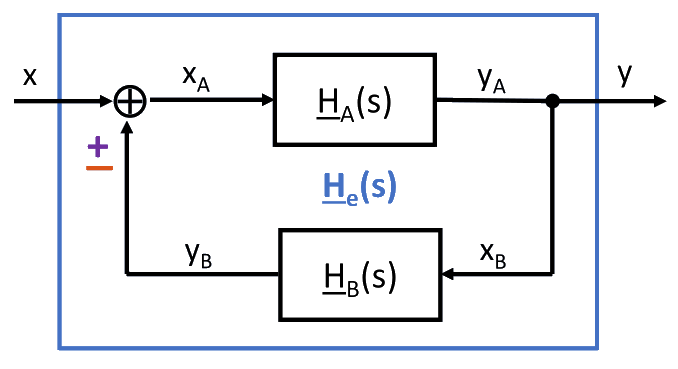
\includegraphics[width=0.6\columnwidth]{Rueckkopplung_Uebertragungsglieder}
    \end{center}
    Beispiel: Kettenschaltung zweier $PT_2$-Glieder ohne Trennverst\"arker.
    \end{itemize}
 
 \subsection{Bode-Diagramm}
 \subsubsection{Merkmale}
 \begin{itemize}
 	\item \textbf{Kettenschaltung LTI-Systeme}
 	
 	\textbf{Addition} der Einzel-Bode-Diagramme beim \par Amplituden- und Phasengang. 
 	
 	\item \textbf{Inverses System}
 	
 	Durch \textbf{Spiegelung} an der x-Achse (Abszisse). 
 \end{itemize}
 
 \subsubsection{Vorgehen}
 \begin{enumerate}
 	\item Ü-Fkt. des LTI-Systems aufstellen.\\
 	Bsp.: Spannungs-Ü-Fkt: $$\underline{H}(s)=\frac{1}{\underline{A}_{11}} = \frac{\underline{U}_2}{\underline{U}_1}$$
 	
 	\item Konstante Faktoren $K$ vor dem Bruch stellen!
 	\item Bauteilelemente in Zeitkonstanten $T=RC$ bzw.  $T=\dfrac{L}{R}$ ausdrücken. {\small $\rightarrow$ Zeitkonstante $T, \tau$ $\neq $ Periodendauer $T$}
 	\item Ü-Fkt. in bekannte Einzelglieder trennen, \\in Normalform mit $T$ ausdrücken $\rightarrow$ siehe Kap. \ref{tabelle_glieder}.\\
 	Bsp.: PDT$_1$-Glied: $$\underline{H}(s)=K\,\frac{1+sT_1}{1+sT_2}$$
 	\item Berechnen der Eck-/Grenzkreisfrequenzen $\omega_0 = \dfrac{1}{T}$ und jeweils im Bode-Diagramm eintragen.
 	\item Amplitudengang:
 	$\underline{H}(s)$ mit $\omega_0=\frac{1}{T}$ \textbf{umformen}:\\ $\Rightarrow$ \textbf{Wichtig}: höchste Potenz von $s$ \textbf{ohne} Vorfaktoren!\\
 	Ersetze $s=j\omega$. \quad Merke:  $\omega\neq\omega_0$.\\
 	
  	Betragsbildung: Zähler und Nenner jeweils Betrag setzen, $j$ fallen lassen.
 	$$ |\underline{H}(\omega)| = \frac{|\underline{Z}|}{|\underline{N}|} = \frac{\sqrt{\text{Re}^2+\text{Im}^2}}{\sqrt{\text{Re}^2+\text{Im}^2}} $$
 	
 	Allgm. Berechnung in $dB$, Grenzfallbestimmung mit: 
 	$$H(\omega) = 20\cdot\log_{10}|\underline{H}(\omega)| \text{ für }\omega=0 \text{ und } \omega \rightarrow \infty $$
 	Zeichnen: Geradennäherung der Glieder in Kap. \ref{tabelle_glieder}.\\
 	
 	Polstelle:  Steigung nach unten $-20db$/Dek.\\
 	Nullstelle: Steigung nach oben $+20db$/Dek.
 	
 	\item Phasengang allgemein:
 	$$\varphi(\omega) = \arctan \left( \frac{\text{Imaginärteil}}{\text{Realteil}} \right)$$
 	Zeichnen: Geradennäherung der Glieder in Kap. \ref{tabelle_glieder}.\\
 	Vorzeichen $\pm K$: Beginn bei $\varphi_{+K}=0$\textdegree \, oder $\varphi_{-K}=180$\textdegree.\\
 	0 bei Null-/Polstelle: $\pm90$\textdegree.\\
 \end{enumerate}
% 1. Übertragungsfunktion aufstellen: H(j!) = U2
% U1
% =
% 1
% A11
% ! gebrochen rationale Funktion
% 2. Das j! durch s ersetzen ! man erhält H(s)
% 3. Konstante Faktoren vor den Bruch ziehen
% 4. Berechnung der Grenzkreisfrequenzen:
% Zähler = 0 ergibt Nullstellen, ! nach s auflösen ! !gx
% Nenner = 0 ergibt Polstellen, ! nach s auflösen ! !gx2
% 5. Übertragungsfunkion H(s) in bekannte Glieder (s. Tabelle) aufteilen (Produkt in Zeitbereich ergibt
% Summe in Bildbereich)
% 6. Berechnung des Amplitudengangs: |H(!)|: Von dein einzelnen Gliedern s wieder durch ! ersetzen,
% und den Betrag bilden (Zähler und Nenner getrennt)
% ���x + zy
% ��� =
% p
% x2 + z2y2
% Logarithmische Skalierung: |H(!)|dB = 20 · log10 |H(!)|
% auch ! ! 0 und ! ! 1 betrachten!
% 7. Berechnen desPhasengangs: '(!): AufteilunginImaginärteilundRealteil
 
 
\end{multicols*}
\begin{center}
	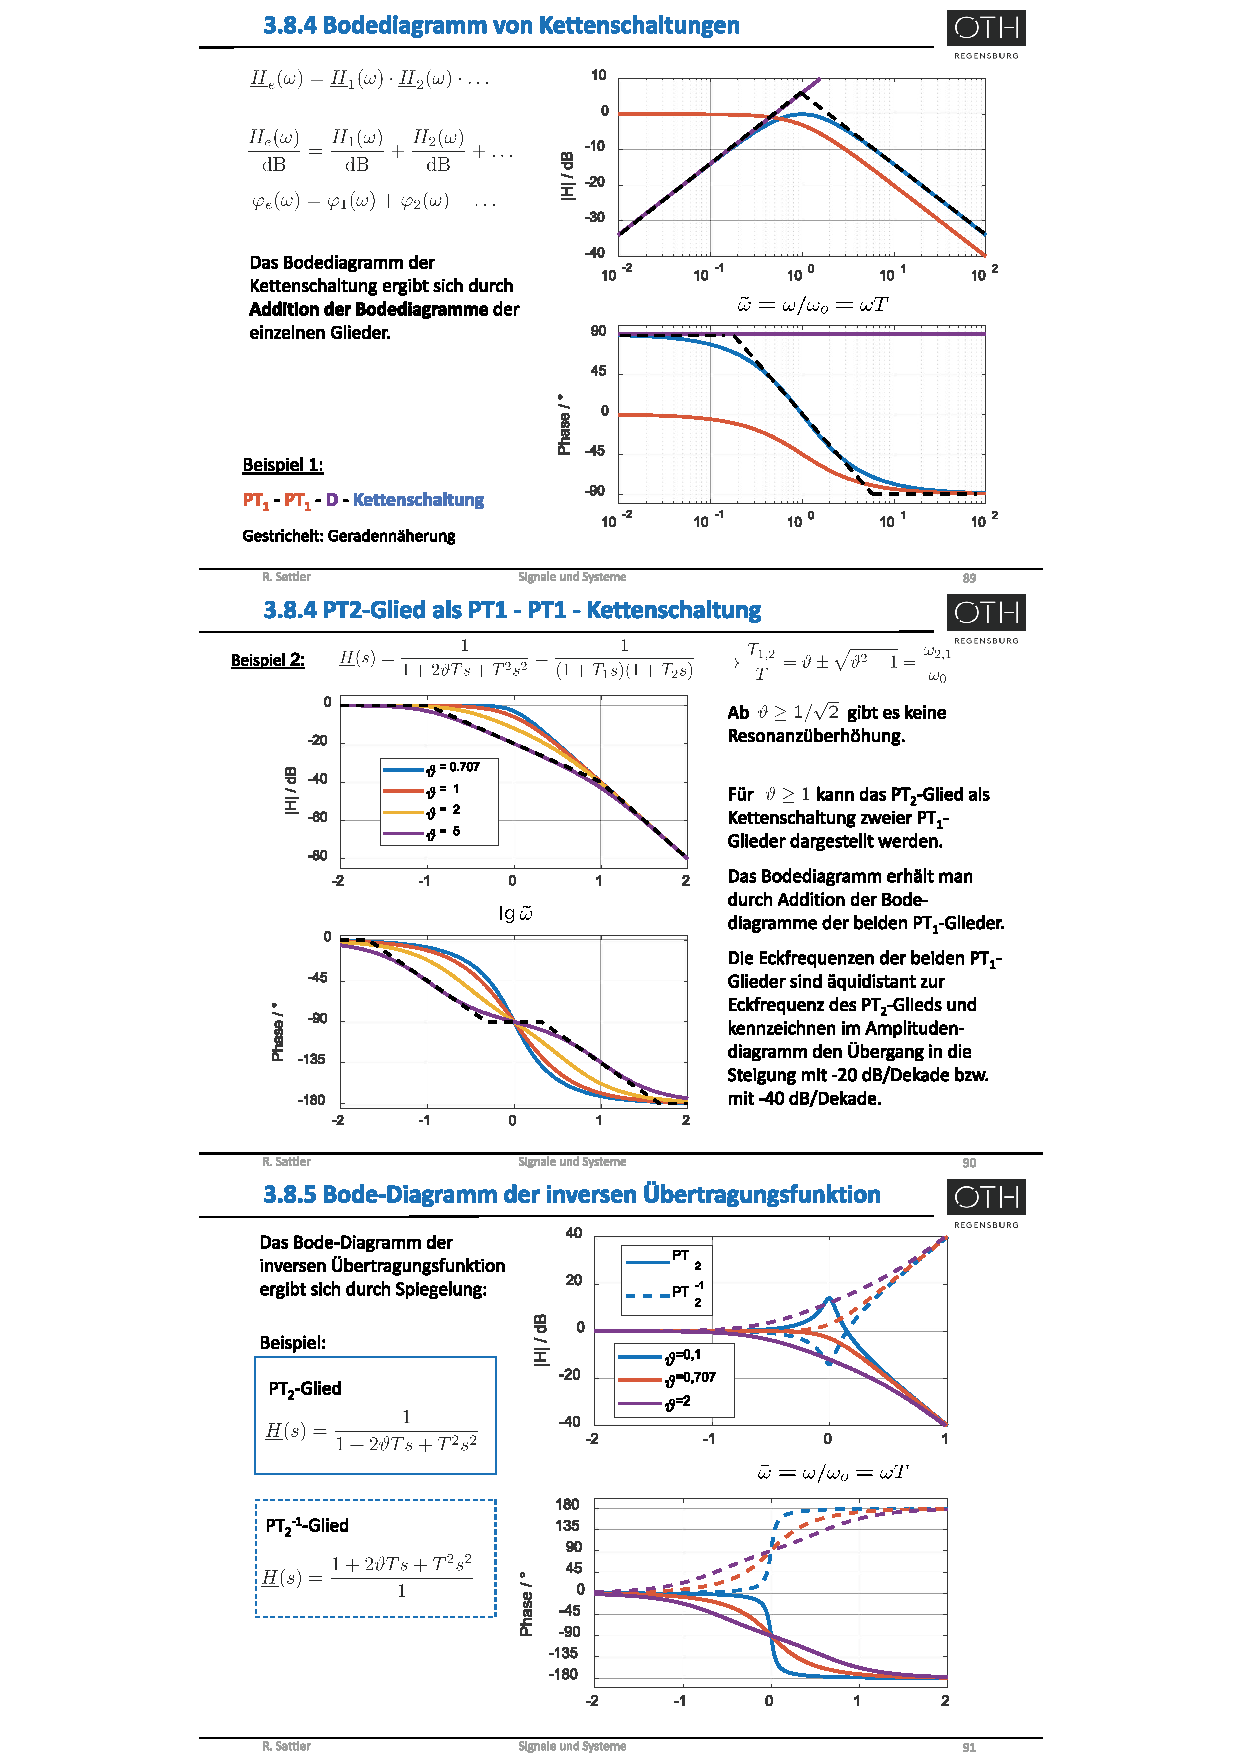
\includegraphics[page=1,width=\textwidth]{Systeme/Bode_Diagramm_Foliensatz}
\end{center}
\subsection{Elementare \"Ubertragungsglieder}
\begin{center}
\raggedright
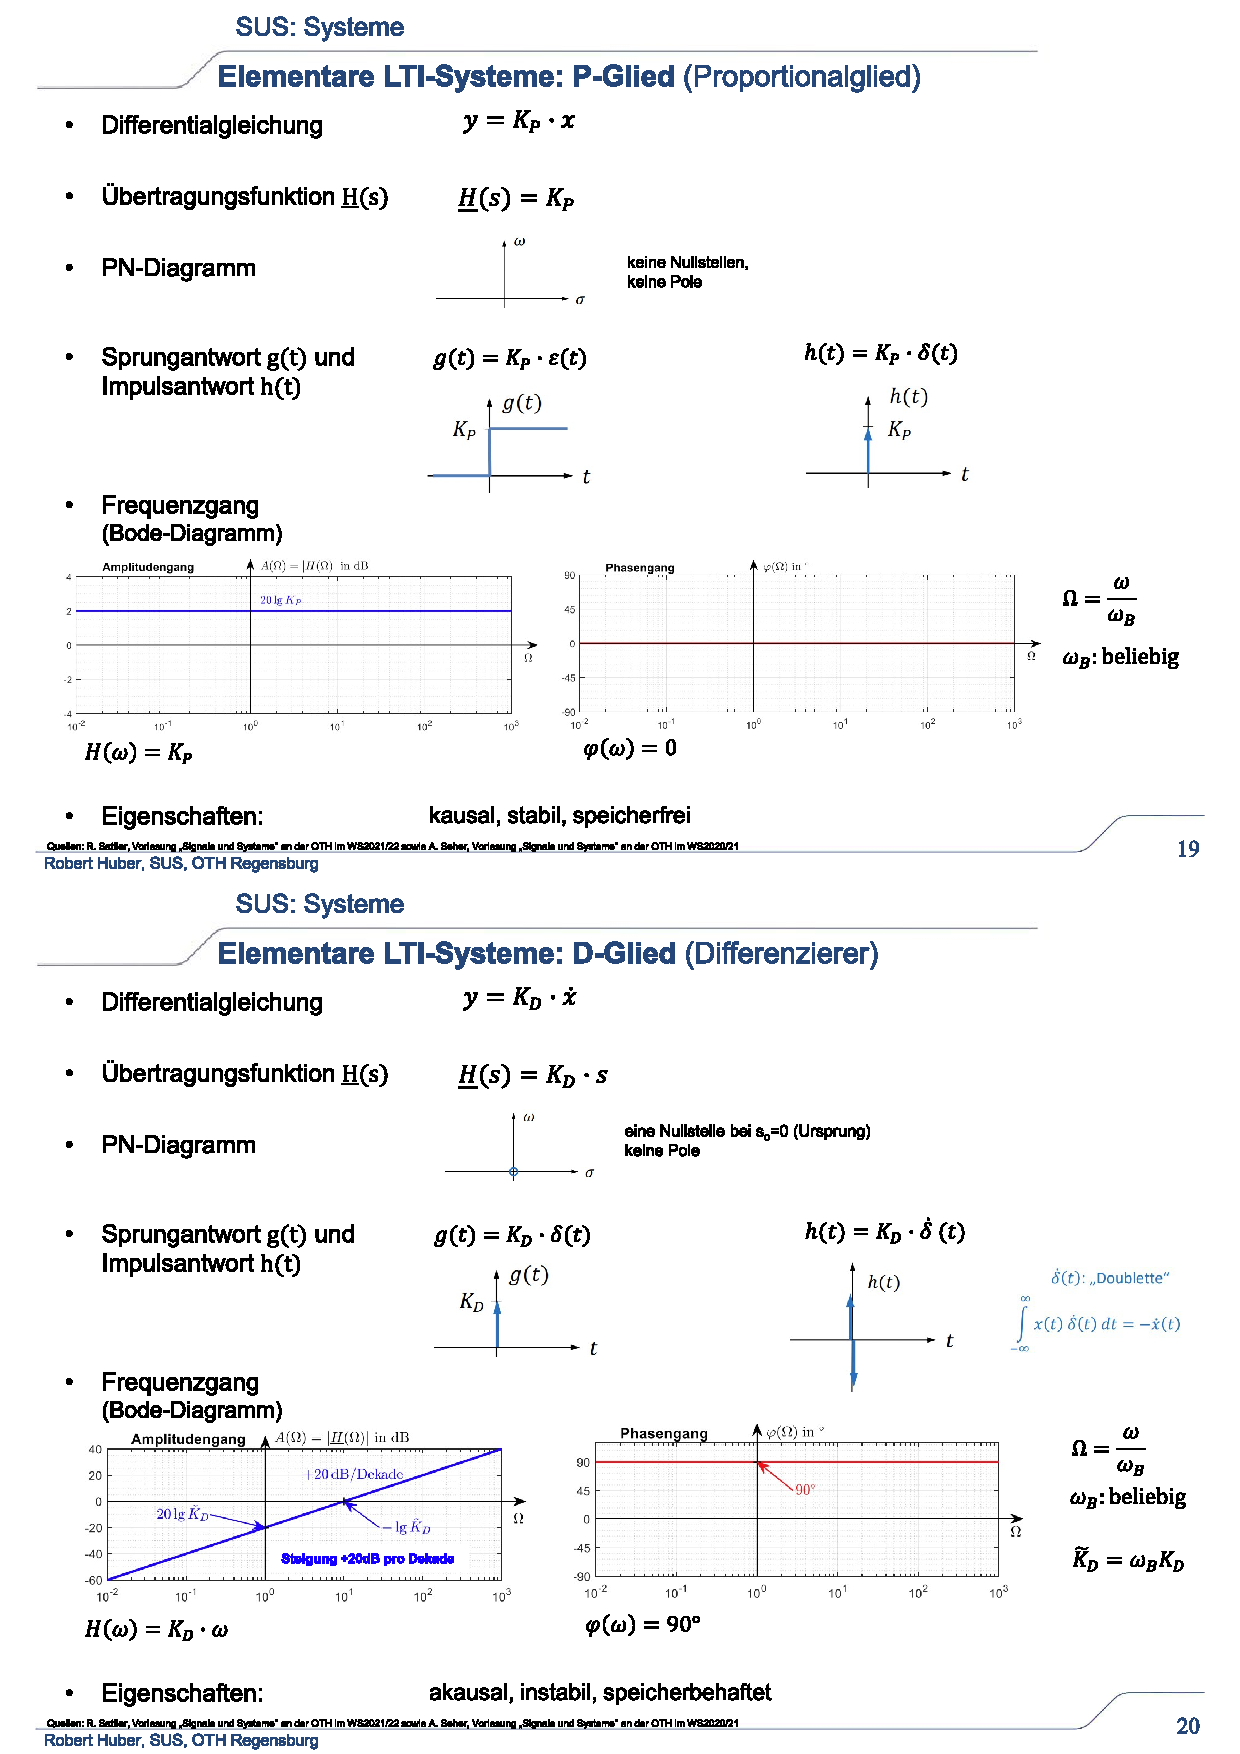
\includegraphics[page=1,width=0.95\columnwidth]{Systeme/GliederHuberEigenschaften}\\
\clearpage
\includegraphics[page=2,width=1\textwidth]{Systeme/GliederHuberEigenschaften}
\includegraphics[page=3,width=1\columnwidth]{Systeme/GliederHuberEigenschaften}
\end{center}

\subsection{Elementare Filter}
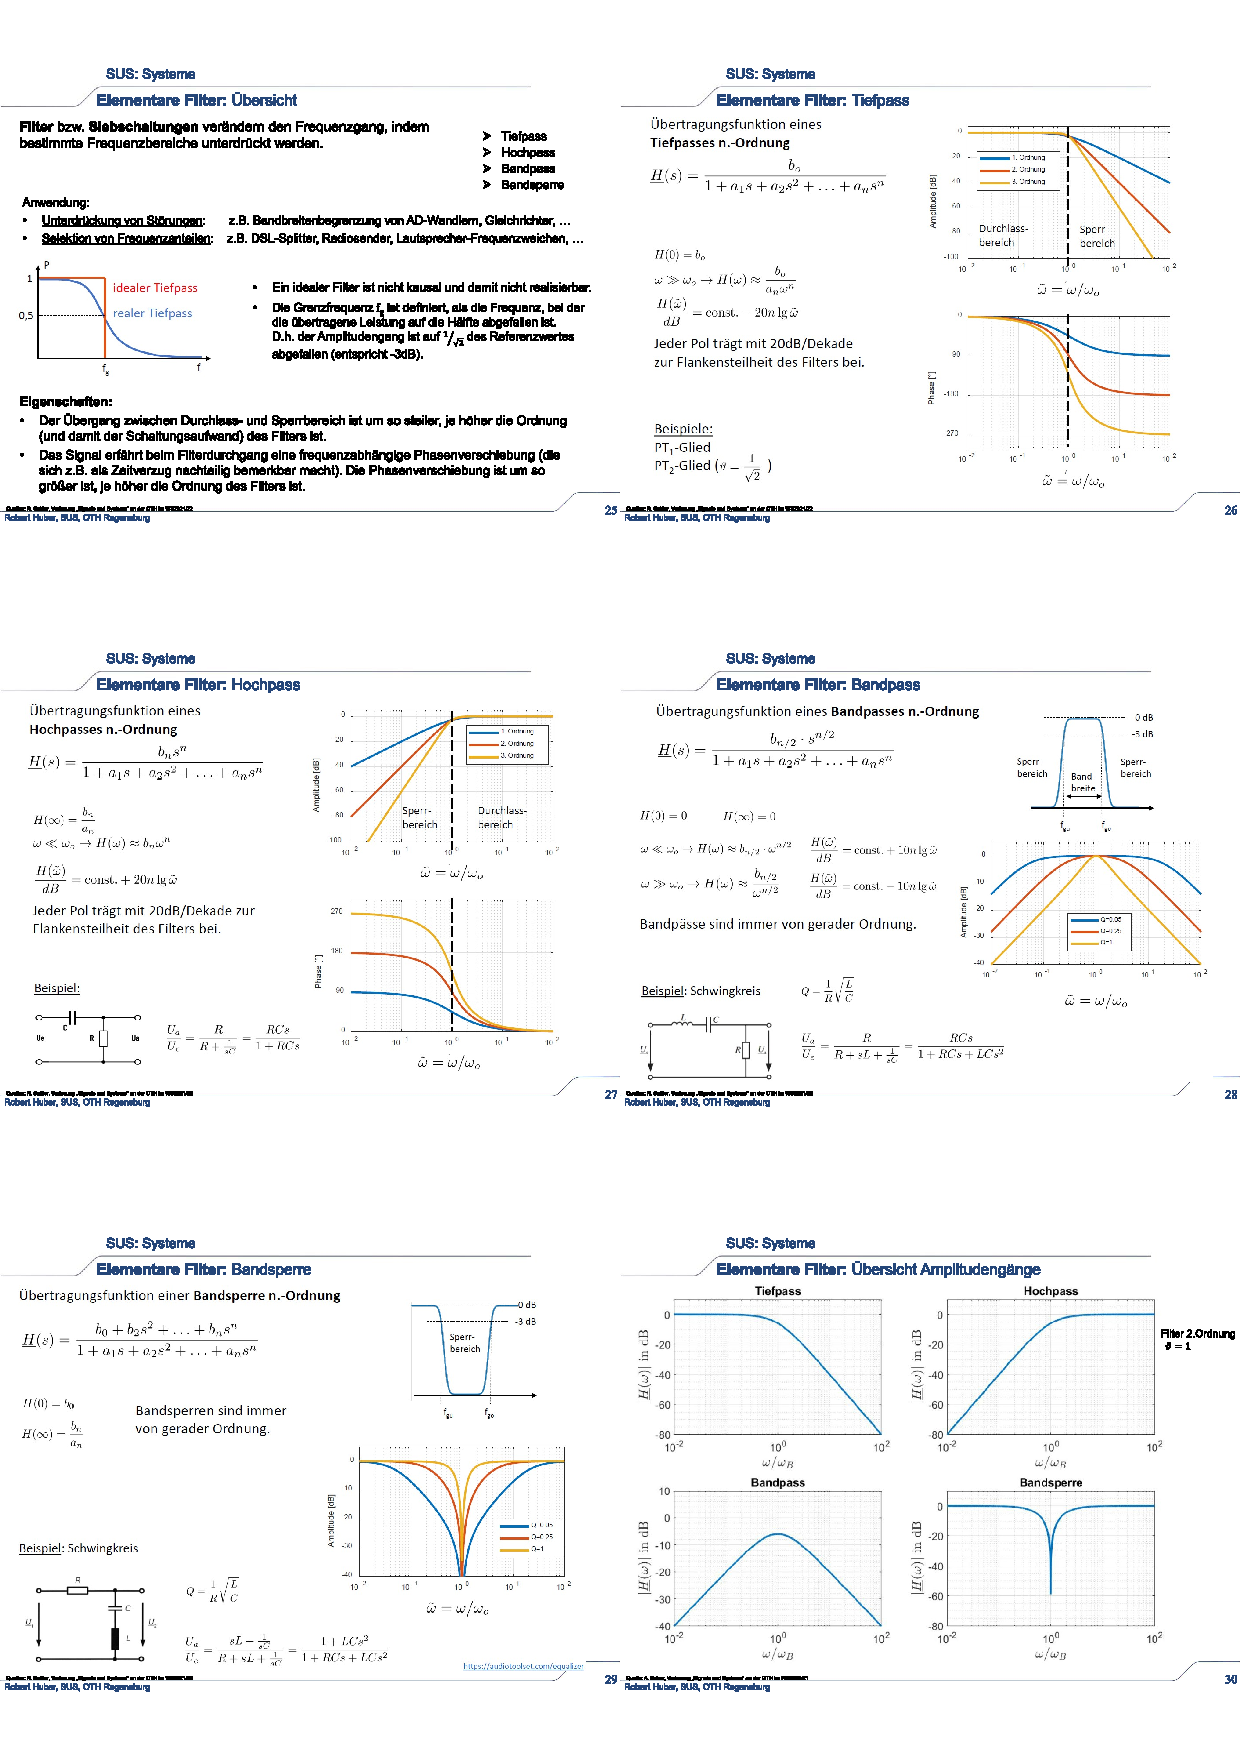
\includegraphics[width=0.97\columnwidth]{Systeme/SUS_Filter_Systeme_Huber}

\subsection{Übersicht wichtiger \"Ubertragungsglieder}\label{tabelle_glieder}
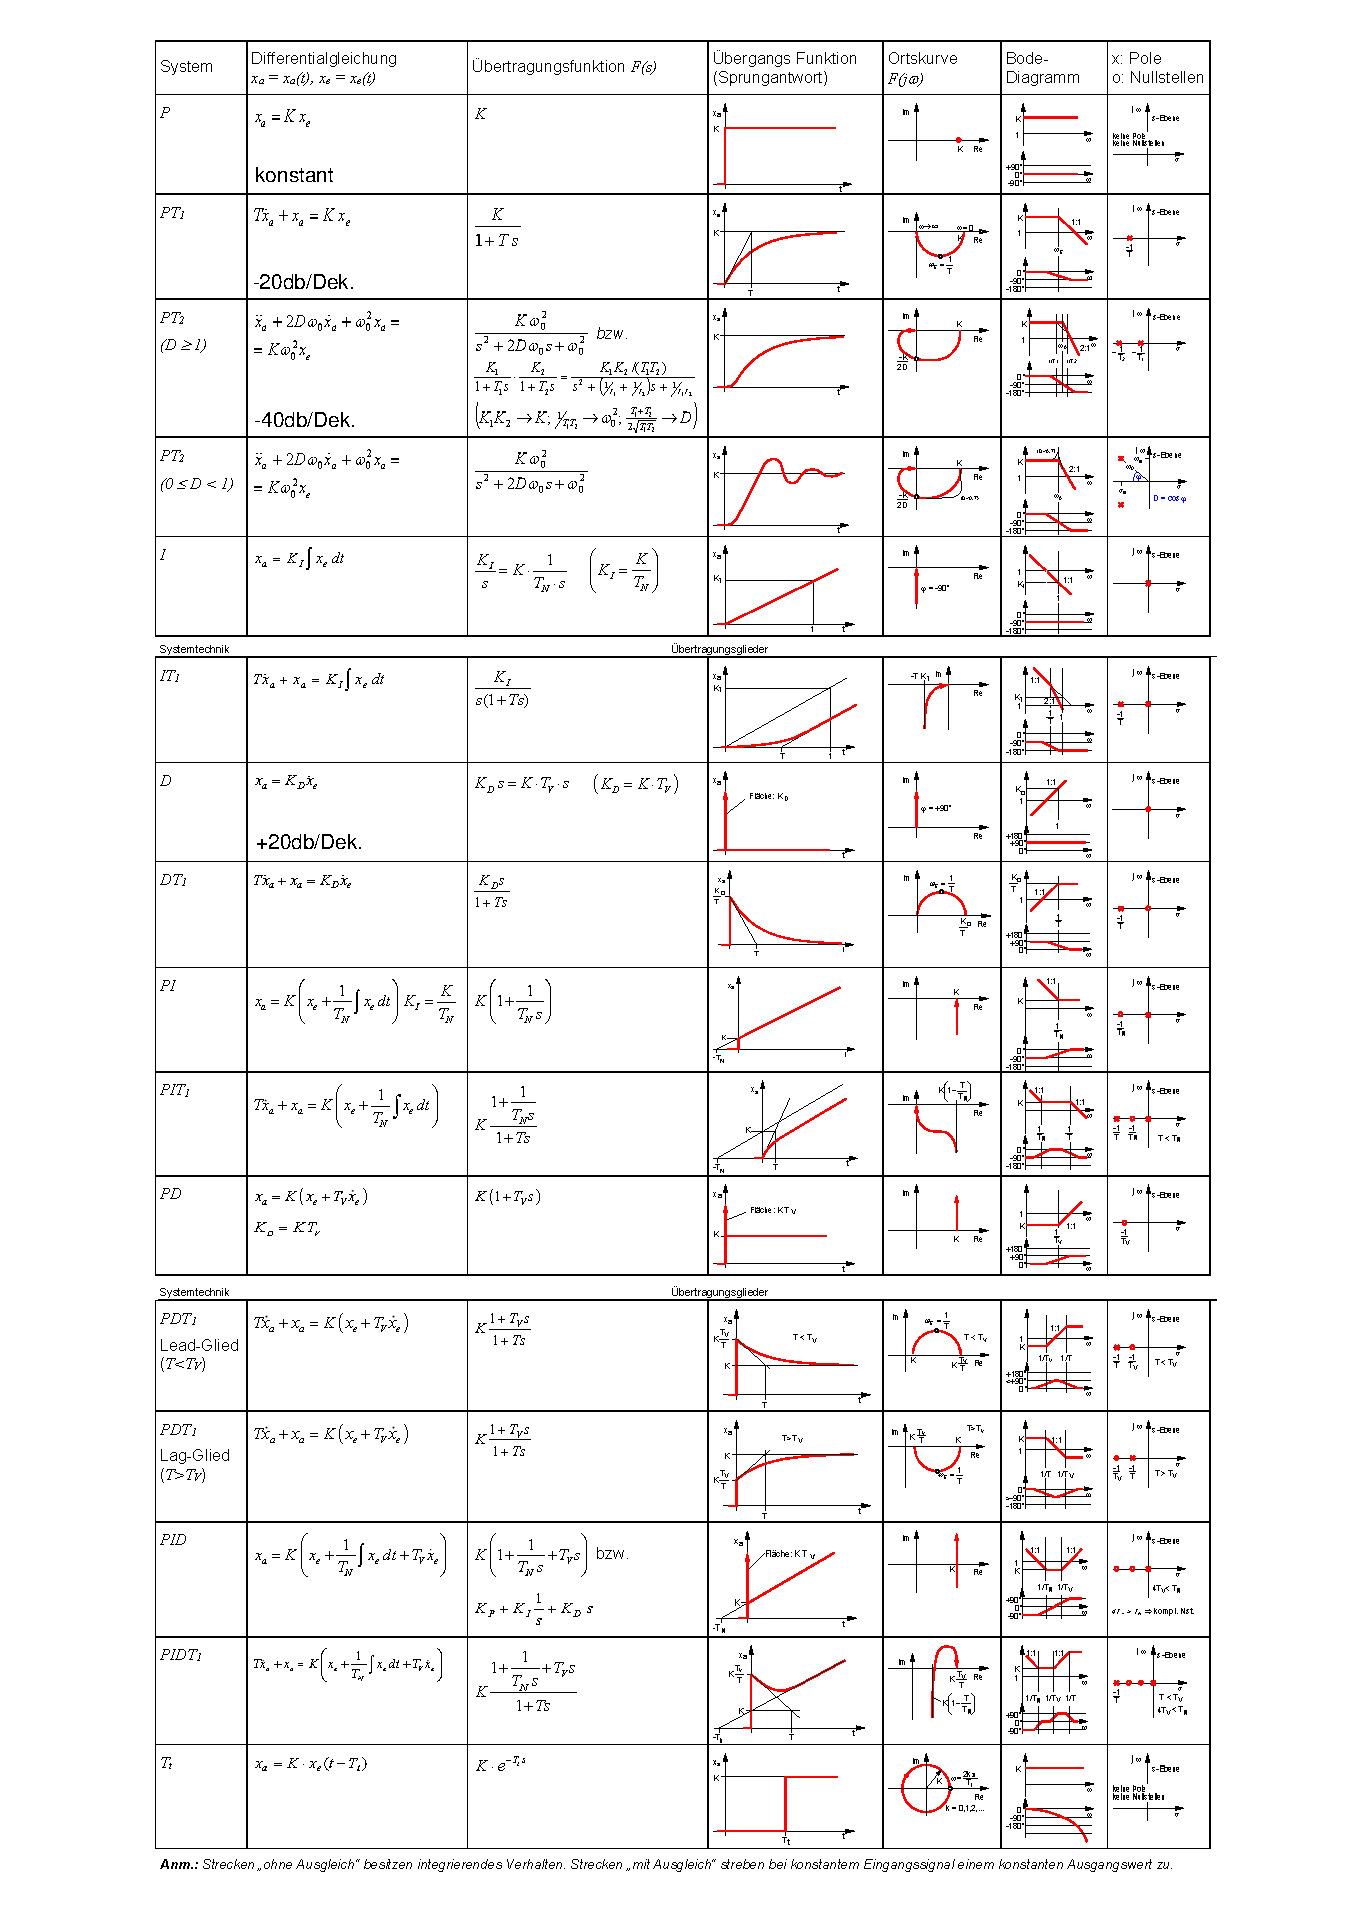
\includegraphics[width=0.82\textwidth]{Systeme/Glieder_Tabelle_mit_Anmerkungen_neu_V3}

\begin{multicols*}{2}




